\providecommand{\econtexRoot}{}
\renewcommand{\econtexRoot}{.}
\providecommand{\econtex}{\econtexRoot/texmf-local/tex/latex/econtex}
\providecommand{\econtexSetup}{\econtexRoot/texmf-local/tex/latex/econtexSetup}
\providecommand{\econtexShortcuts}{\econtexRoot/texmf-local/tex/latex/econtexShortcuts}
\providecommand{\econtexBibMake}{\econtexRoot/texmf-local/tex/latex/econtexBibMake}
\providecommand{\econtexBibStyle}{\econtexRoot/texmf-local/bibtex/bst/econtex}
\providecommand{\notes}{\econtexRoot/texmf-local/tex/latex/handout}
\providecommand{\handoutSetup}{\econtexRoot/texmf-local/tex/latex/handoutSetup}
\providecommand{\handoutShortcuts}{\econtexRoot/texmf-local/tex/latex/handoutShortcuts}
\providecommand{\handoutBibMake}{\econtexRoot/texmf-local/tex/latex/handoutBibMake}
\providecommand{\handoutBibStyle}{\econtexRoot/texmf-local/bibtex/bst/handout}

  
\documentclass[titlepage]{\econtex}\providecommand{\texname}{Dissertation-Proposal}


\providecommand{\EqDir}{Equations}
\providecommand{\FigDir}{Figures}
\providecommand{\CodeDir}{Code}
\providecommand{\CalibrationDir}{Calibration}
\providecommand{\TableDir}{Tables}
\providecommand{\ApndxDir}{Appendices}

\usepackage{subfiles}

\providecommand{\onlyinsubfile}{}
\providecommand{\notinsubfile}{}
\renewcommand{\onlyinsubfile}[1]{}
\renewcommand{\notinsubfile}[1]{#1} 


\usepackage{\econtexSetup}\usepackage{\econtexShortcuts}\usepackage{makecell} 
\renewcommand{\util}{\mathrm{u}}
% replace PF-FHWC with just FHWC
\renewcommand{\InvEpShkInv}{\hat{\pShk}}
%\renewcommand{\InvEpShkInv}{\check{\pShk}}
\renewcommand{\PGroAdj}{\hat{\PGro}}
\renewcommand{\PatPGroAdj}{\text{\pmb{\Thorn}}_{\PGroAdj}}
% get rid of \DiscAlt
\renewcommand{\PGrouAdj}{\ensuremath{\hat{\hat{\PGro}}}}
\renewcommand{\pGrouAdj}{\ensuremath{\hat{\hat{{\pGro}}}}}
\renewcommand{\DiscAltuAdj}{\ensuremath{\hat{\hat{\beth}}}}
\renewcommand{\uInvEpShkuInv}{\hat{\hat{\psi}}}
\renewcommand{\pNotZero}{(1-\pZero)}
\providecommand{\YLevBF}{\ensuremath{\mathbf{Y}}}


\provideboolean{Shorter}
\setboolean{Shorter}{true}
\setboolean{Shorter}{false}
\providecommand{\ShorterYN}{\ifthenelse{\boolean{Shorter}}}
\usepackage{rotating}\usepackage{subfigure}


\hypersetup{pdfauthor={William Du <wdu9@jhu.edu>},
            pdftitle={Dissertation Proposal},
            pdfkeywords={Heterogenous Agents, marginal propensity to consume, Nominal Rigidities, buffer-stock saving, permanent income hypothesis},
            pdfcreator = {wdu9@jhu.edu}
}

\begin{document}\bibliographystyle{\econtexBibStyle}
\renewcommand{\onlyinsubfile}[1]{}\renewcommand{\notinsubfile}[1]{#1} 

\hfill{\tiny \texname.tex, \today}

\begin{verbatimwrite}{\texname.title}
Theoretical Foundations of Buffer Stock Saving
\end{verbatimwrite}


\title{Unemployment Expectations, Precautionary Savings, and the Business Cycle}

\author{William Du\authNum}



\keywords{Beliefs, Precautionary Saving, Heterogeneous Agents, Incomplete Markets, Search and Matching}




\maketitle 


\hypertarget{abstract}{}
\begin{abstract}
This dissertation proposes studying how the quantitative consequences of precautionary savings over the business cycle differ when using expectations data on job transition probabilities to discipline a model of counter cyclical unemployment risk.
\end{abstract}


\begin{authorsinfo}
\name{Contact: \href{mailto:wdu9@jhu.edu}{\texttt{wdu9@jhu.edu}}}
\end{authorsinfo}

\thanks{ }

\titlepagefinish


\newtheorem{defn}{Definition}
\newtheorem{theorem}{Theorem}

\hypertarget{Introduction}{}
\section{Introduction}

\label{sec:intro}



The past decade has seen an eruption of research on the importance of household uncertainty over the business cycle. Empirically, increases in various measures of household uncertainty, such as income risk or consumer sentiment of future economic conditions, have shown to generate fluctuations in aggregate activity\footnote{\cite{bayer2019precautionary} show that a one standard deviation increase in income risk decreases aggregate activity by 0.2 percent.  \cite{leduc2016uncertainty} construct of measure of uncertainty using survey data from the Michigan Survey of expectations to show that increases in their measure raises unemployment and lowers inflation}. More convincingly, in a randomized control trial framework, recent work by \cite{coibion2021effect} establishes that higher uncertainty (uncertainty in GDP forecasts) \textit{causes} households to sharply reduce spending.  Theoretically, the literature has calibrated structural models to demonstrate that heightened uncertainty, in the form of increased income risk or unemployment risk, can generate sizable business cycle dynamics and amplify shifts in aggregate demand \footnote{ Some examples include \cite{bayer2019precautionary}, \cite{mckay2017time} ,\cite{ravn2017job}}. In these models, the effects of uncertainty largely stem from the precautionary motive: heightened uncertainty induces households to increase savings and reduce consumption. Indeed the precautionary savings channel has been empirically documented to be the second most important factor behind the decline in aggregate consumption in the US during the Great Recession (\cite{carroll2012dissecting}) and in other work the most important factor in the decline in global consumption (\cite{mody2012precautionary}) during the same period. Although precautionary savings operate through households expectations of their future income, no work has yet to use expectations data to quantify the role of precautionary savings. Considering the expansive literature on beliefs and the surrounding biases in the formation of expectations, the quantitative implications of the precautionary savings channel may differ substantially between a model disciplined by expectations data and its rational expectations counterpart. For instance, using expectations data on job transition probabilities, \cite{mueller2021job} find job seekers to underreact in their job finding expectations to changes in the actual job finding probability, suggesting persistence or, according to \cite{menzio2022stubborn}, stubborness in their job finding expectations.  If expectations on job finding probabilities are stubborn and underreact to gradual increases in the true job finding probability, say at the trough of the business cycle, after a large negative output shock, then a model of countercyclical unemployment risk with beliefs on job transition probabilities would produce more persistent responses in aggregate consumption in comparison to the same model without beliefs as stubborn beliefs would cause households to hold a larger precautionary buffer stock for longer. Therefore, using expectations data to calibrate a model of precautionary savings may have substantially different quantitative implications. \\

In my job market paper, I aim to understand how the quantitative consequences of unemployment risk differ when introducing expectations data on job transition probabilities to discipline a model of counter cyclical unemployment risk. In particular, since the effects of unemployment risk work through the precautionary motive\footnote{Increases in job separation probabilities (decreases in job finding probabilities) induce households to reduce consumption and increase savings}, I look to quantify the role of the precautionary savings in explaining the difference between fluctuations produced by a model augmented with beliefs on job transition probabilities and its rational expectations counterpart. For the moment being, the goal is to capture the quantitative implications of biases inherent in the expectations data and how they influence precautionary savings to induce business cycle fluctuations instead of taking a theoretical stance on how or why these biases are formed. \\

I plan to solve an extension of \cite{broer2021unemployment}'s Heterogeneous Agent New Keynesian(HANK) model with Search and Matching(SAM) frictions by including beliefs on job transition probabilities and permanent and transitory income shocks. In the model, households face uninsurable permanent and transitory income shocks as well as stochastic unemployment risk dictated by job finding and job separating probabilities.The true job transition probabilities are unobserved by households and instead households form beliefs on these probabilities. I do not not take a stance on how beliefs are formed theoretically. Beliefs will be updated according to an empirical relationship between the expectations data on job transition probabilities and the actual job transition probabilities. The aim is to capture what the expectations data implies as opposed to how households form expectations on job transition probabilities. The addition of search and matching frictions not only provide a foundation to accommodate expectations data on job transition probabilities but also allow for a micro-founded model of counter-cyclical unemployment risk. The HANK and SAM literature has documented that the interaction between risk aversion, nominal rigidities, and search frictions produces counter cyclical unemployment risk that amplifies fluctuations in aggregate demand. Intuitively, a fall in output reduces labor demand which in turn reduces the number of vacancies leading job finding probabilities to fall and job separating probabilities to rise inducing a precautionary savings motive that causes a further decline in consumption and, equivalently, output. This theory is in fact consistent with the work of \cite{leduc2016uncertainty}, who find that the effects of macroeconomic uncertainty operate partly through an aggregate demand channel and the findings of \cite{guvenen2014nature}, who document that earnings growth exhibits pro-cyclical skewness implying severe negative events are more likely during recessions. \\

Given the importance of aggregate demand in the transmission of the precautionary channel, it is vital to have a model that produces realistic fluctuations in aggregate consumption. This motivates the inclusion of permanent and transitory shocks to generate a distribution of wealth featuring serious heterogeneity that can be calibrated to match the empirical distribution of wealth. Recent research in the HANK literature has emphasized the importance of the distribution of wealth in producing realistic fluctuations in aggregate consumption\footnote{\cite{auclert2018intertemporal}, \cite{patterson2019matching} ,\cite{kaplan2018monetary}}. For instance, \cite{auclert2018intertemporal}  emphasize the role of the intermediately constrained households (households that are nearly hand to mouth) in generating persistence in the dynamics of aggregate consumption that cannot be replicated by a TANK model. Further, \cite{auclert2019monetary} establishes the existence of redistribution channels in the transmission of monetary policy exclusive to HANK models. Confirming the empirical significance of this channel by using administrative data from Denmark, \cite{crawley2020consumption} demonstrate some of these redistributive channels to be substantially more important in explaining consumption growth than the intertemporal substitution channel. In a structural model, the strength of these redistributive channels are functions of the cross sectional distribution of MPCs and therefore the cross sectional distribution of wealth. Moreover, \cite{heathcote2018wealth} show that households with lower liquid wealth exhibit increased sensitivity in their precautionary motive when faced with heightened unemployment risk. In summary, the distribution of wealth plays an essential role in shaping the response of aggregate consumption and thus the share of the precautionary motive. \\

The core contribution of this project is the use of expectations data to quantify the role of unemployment expectations, and therefore precautionary savings, in its ability to explain fluctuations over the business cycle. To the best of my knowledge, this paper would be the first to do so. The results of this project may motivate the management of unemployment expectations in the design of stabilization policy, especially if these expectations are subject to pervasive biases that amplify business cycle fluctuations. Indeed, unemployment expectations have been shown to be robustly correlated with spending (\cite{carroll1997unemployment}). Further, \cite{pedemonte2020fireside} demonstrates that during the Great Depression regions of America with increased exposure to President Roosevelt's fireside chats saw significant increases in spending on durable goods. This is notable as Roosevelt's fireside chats highlighted the introduction of unemployment benefits and other New Deal Legislation suggesting the importance of managing unemployment expectations on stimulating consumer behavior. \\

The rest of the paper is as follows. Section 2 details a literature review. Section 3 describes the data. Section 4 presents a preliminary model to be disciplined by expectations data. Section 5 details my next steps in the research process and finally section 6 details possible interesting extensions. 




\hypertarget{Literature Review}{}
\section{Literature Review}


The core contribution of this project is to the HANK and SAM literature. The literature on HANK and SAM emphasizes the interaction between nominal rigidities, search frictions, and incomplete markets to generate counter-cyclical unemployment risk, and thus countercyclical precautionary savings, that amplify changes in aggregate demand  (\cite{den2018unemployment}, \cite{leduc2016uncertainty}, and \cite{ravn2017job}). For instance, using an estimated quantitative HANK and SAM model, \cite{challe2017precautionary} demonstrate the significance of this precautionary channel by illustrating that the fall in aggregate consumption during the Great Recession would have been 1.75 times smaller without the effects of precautionary savings (-3.5 percent drop in consumption in the data, and they find a -2 percent drop in their counterfactual experiment without precautionary savings). With respect to how HANK and SAM models influence monetary policy, \cite{challe2020uninsured} finds that negative supply shocks call for interest rate cuts due to the amplifying effect of precautionary savings on aggregate demand.  Moreover, \cite{gornemann2016doves} find that households prefer policy focused on unemployment stabilization even if it incurs deviations from price stability due to the amplifying effects of precautionary savings. In regards to quantifying unemployment risk, \cite{broer2021unemployment} add endogenous job separations (typically assumed exogenous in this literature) and sluggish vacancy creation to a HANK and SAM model to produce empirically consistent co-movements between job transition probabilities and to quantify the unemployment risk channel: the difference in the response of unemployment between a model with incomplete markets and and a model with complete markets. They find the unemployment risk channel to account for 35 percent of the variance in unemployment after a TFP shock. Effectively, the unemployment risk channel, as they define it, is the consequence of precautionary savings and therefore their paper is closest to this project. In contrast to \cite{broer2021unemployment}, I look to quantify how the consequences of precautionary savings differ when using expectations data. In addition, since countercyclical income risk operates through aggregate demand to amplify unemployment risk, the response of aggregate consumption is crucial in quantifying this channel. Therefore this project necessitates a model of realistic household behavior with thorough heterogeneity as the HANK literature has shown the importance of the distribution of wealth in explaining fluctuations in aggregate consumption. Few HANK and SAM models generate meaningful heterogeneity across the distribution of wealth. Instead, the literature on countercyclical income risk makes strong assumptions to allow for a degenerate distribution of wealth for tractability and transparency in the mechanisms within the model. Overall, I contribute to the HANK and SAM literature by introducing expectations data on job transition probabilities to quantify the underlying precautionary savings channel/unemployment risk channel that dictates all its results and by being the second paper (first paper to do so is \cite{gornemann2016doves}) to introduce a realistic model of household behavior to the HANK and SAM framework.




\hypertarget{Data}{}
\section{Data}

The expectations data on job finding and job separating probabilities are gathered from the Survey of Consumer Expectations and the Michigan Survey of Expectations(MSE). The Survey of Consumer Expectations (SCE) is a nationally representative, Internet-based survey of a rotating panel of approximately 1,300 household heads. The survey tracks a respondent's age, income, education, homeownership status, employment history, and region. The data spans from June 2013 to the present at a monthly frequency. The SCE contains expectations on job finding probabilities at a three month horizon and expectations on job losing probabilities at a one year horizon. In addition, expectations of job loss probabilities within 4 months are available however only at a 4 month frequency beginning in July of 2014. The Michigan Survey of Expectations is also a nationally representative survey that conducts 500 interviews by telephone each month.  The MSE provides expectations of job loss within 5 years at a monthly frequency beginning in December 1997. I hope to calibrate my model to a quarterly frequency so I will need to obtain a time series of 3 month job loss expectations. Using all the job loss expectations data at differing horizons from both the MSE and the SCE and other macroeconomic time series such as the unemployment rate and stock market indices, I plan to impute the implied job loss expectations at a 3 month horizon. This will be a separate empirical project I will pursue with a fellow classmate. \\

The actual job finding and job separating probabilities are to be estimated using \cite{shimer2012reassessing}'s method with data from the Current Population Survey (CPS) under the Bureau of Labor Statistics (BLS).  So far, I have computed the one month job finding and job separation probabilities at a monthly frequency using \cite{shimer2012reassessing}'s baseline method however they will need to be recomputed. In my computation, I obtain a negative job finding probability for the month of April 2020 which saw an unprecedented surge in unemployment. My original computation uses Shimer's baseline method which assumes that workers only transition between employment and unemployment. When Shimer extends his method to assume that workers may also transition out of the labor force, he demonstrates the time series data on job finding and job separation yields no substantial difference in comparison to their counterparts in the baseline method. Because the baseline method is much more tractable he advocates for that method. However, I hypothesize that a large number of workers may have transitioned from out of the labor force into unemployment to receive unemployment benefits and that may have yielded a negative job finding probability. Thus, I plan on recomputing the job finding and job separation probabilities to include transitions out of the labor force. Therefore, for the time being, I exclude April 2020 from my one month job finding and job separating time series. \\

\begin{figure}{}
    \centering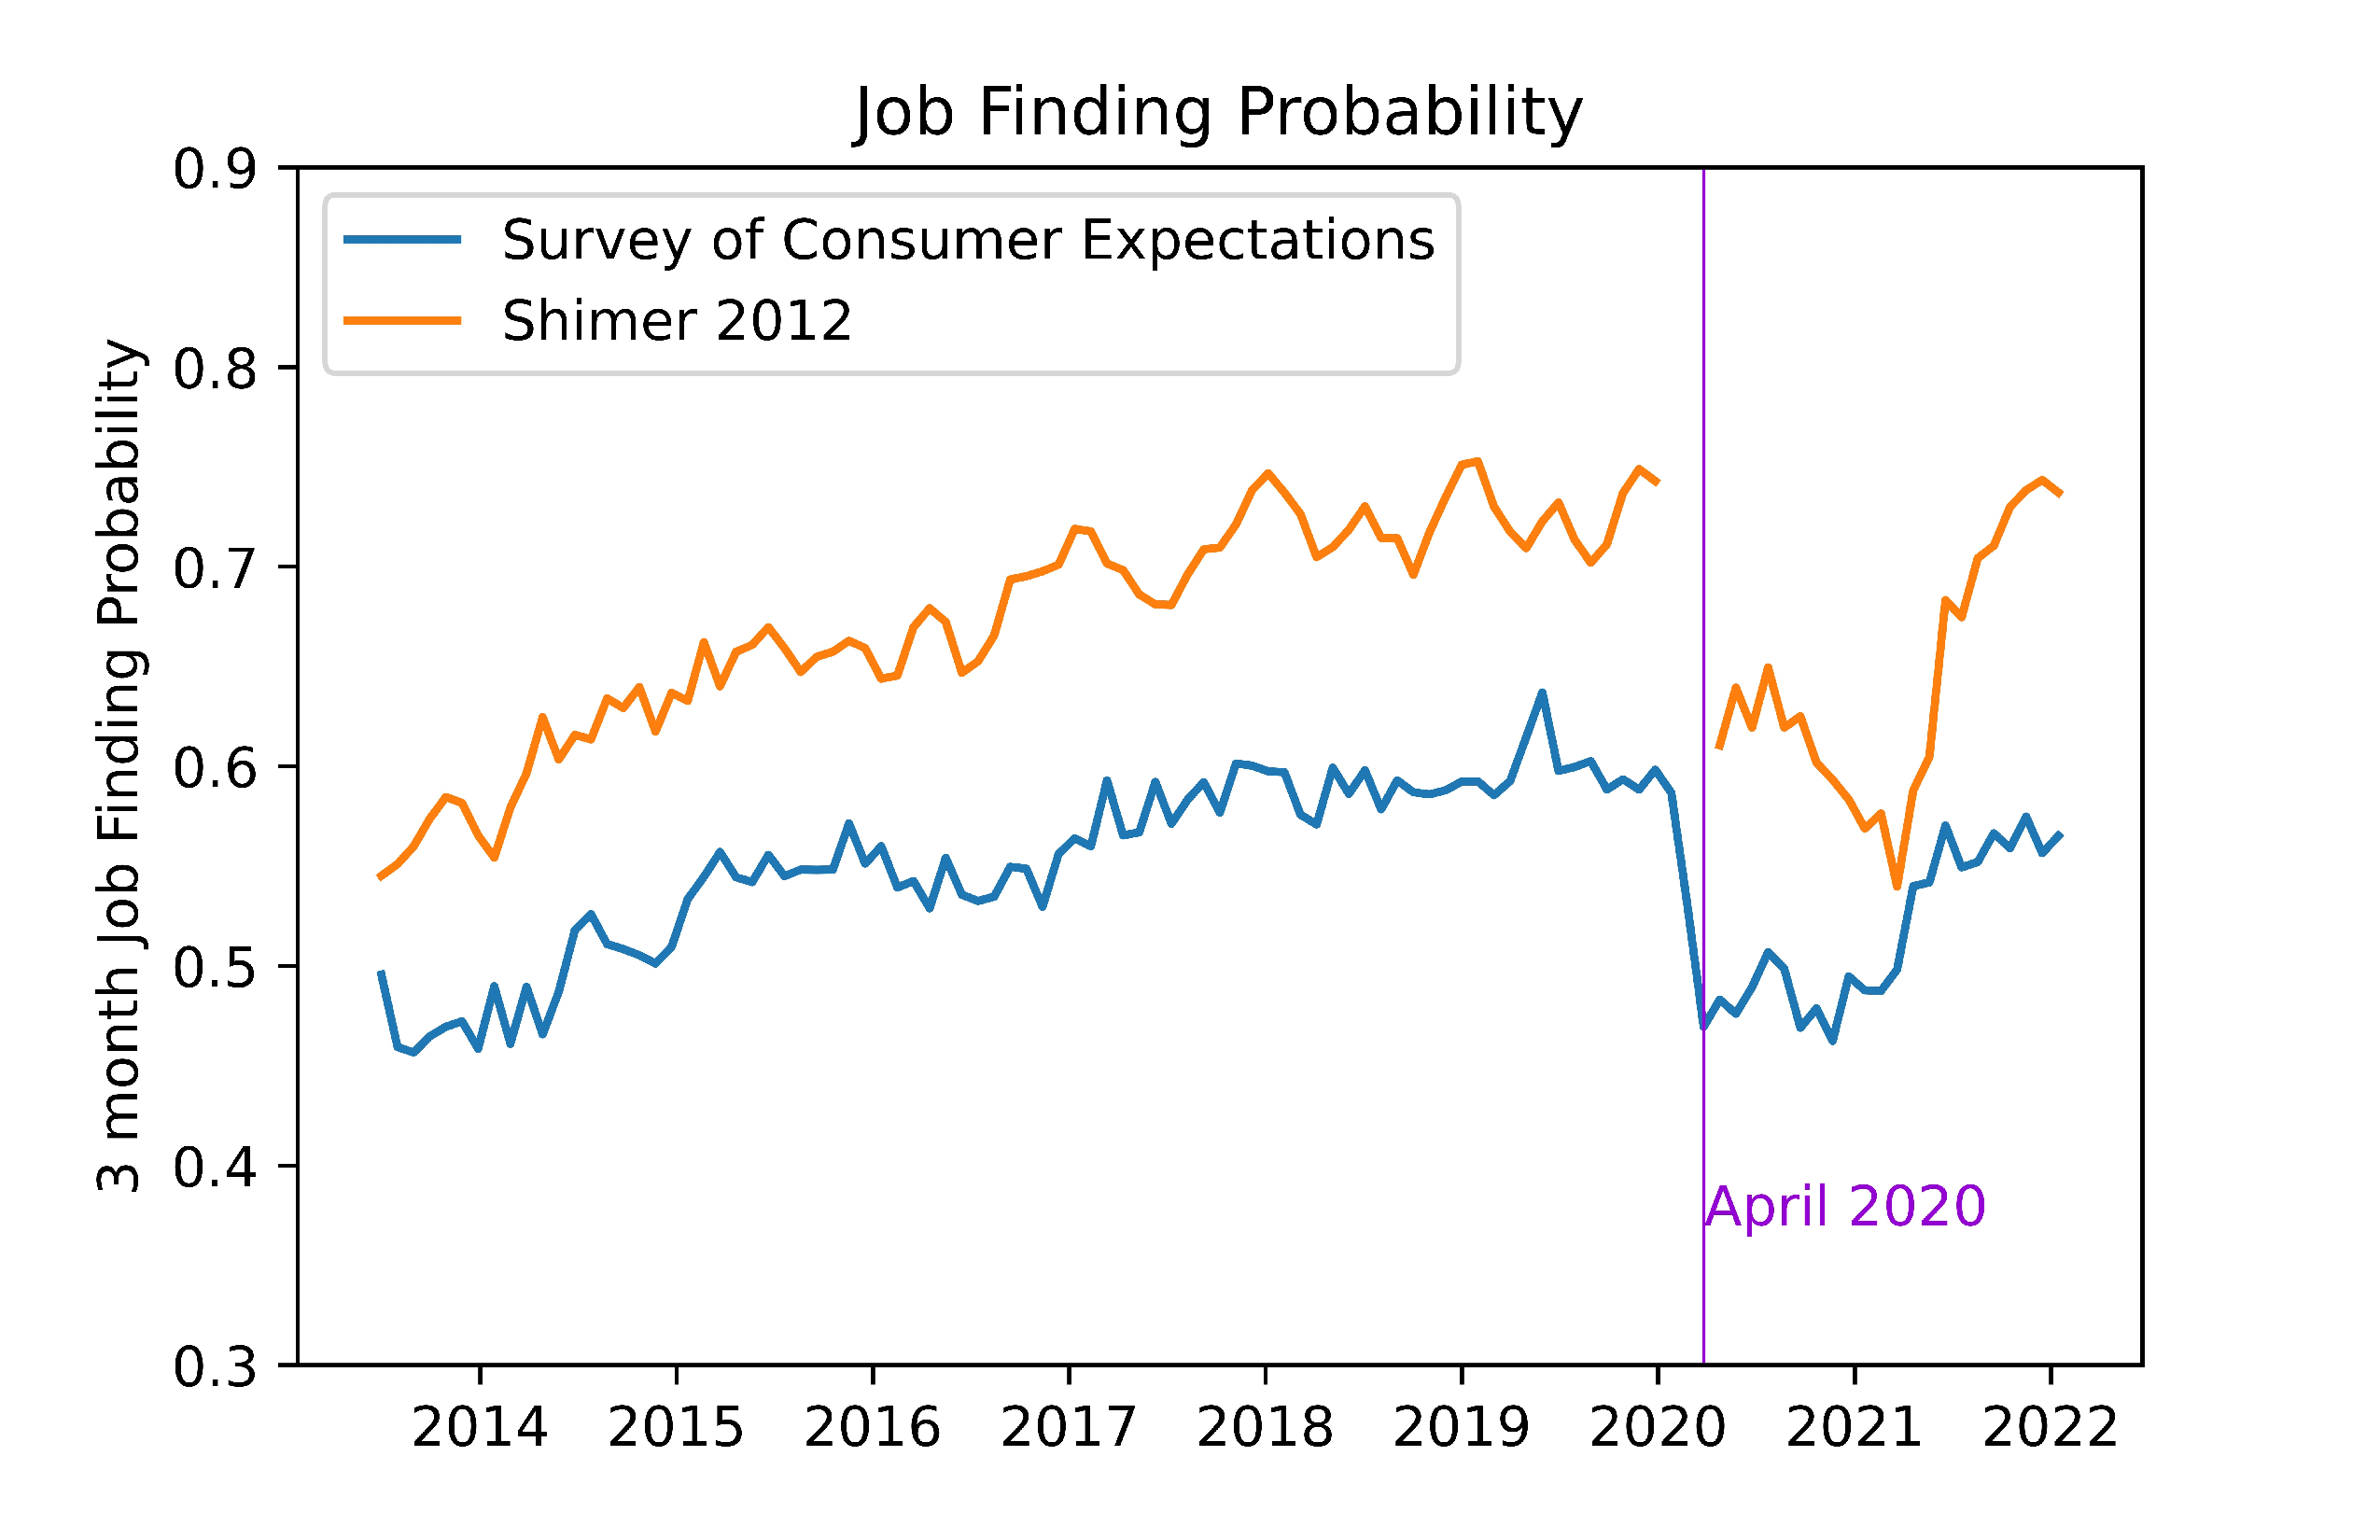
\includegraphics[scale=.26]{\FigDir/JF}
    \caption{Comparison of expectations of 3 month job finding  against the actual 3 month job finding probability. }
\end{figure} 



A plot of the actual 3 month job finding probability and the expectation of the 3 month job finding probability are found in figure 1. The actual 3 month job finding probability is constructed using the observed one month job finding probabilities. Since the one month series is missing the month of April, a few observations around April 2020 are missing as each 3 month job finding observation requires 3 one month job finding observations. The figure displays a level difference and a seemingly strong correlation. Given that I am interested in fluctuations over the business cycle, the difference in the changes exhibited by the series is of focus. \\



\begin{figure}{}
    \centering\includegraphics[scale=.26]{\FigDir/JS}
    \caption{Comparison of 5 month moving average of expectations of 1 year job separating probability against the actual 1 year job separating probability. }
\end{figure}



\begin{figure}{}
    \centering\includegraphics[scale=.26]{\FigDir/JS2}
    \caption{Comparison of raw expectations data of 1 year job separating probability, its 5 month moving average, and  the actual 1 year job separating probability. }
\end{figure}




More interestingly, in figure 2, a plot of the 5 month moving average of the  one year job separating expectations are presented against the realized one year job separating probability computed using \cite{shimer2012reassessing}'s method. For the series of actual job separation probabilities, I exclude observations during and after the pandemic because the job separation probabilities are derived from the job finding probabilities and thus many observations after the pandemic are missing. I focus on the correlation between both time series because I plan to have job separation expectations evolve according to a regression of the expectations on the realized values and likely their lags values as well.  Therefore the level difference between the time series will not matter as it will be captured by the intercept. Looking at the time series, beginning in early 2016, both series display a hump shape that rises and eventually falls back to its trend. For the expectations data, this hump lasts for at least a year while the the realized job separation data exhibits a much smaller hump that returns to its trend more quickly. This suggests that during this period, households were more pessimistic in the change in their probability of being fired compared to the actual data. In other words, households believed that the probability of losing a job had increased more than the actual job finding probability had increased. Overall, although the changes, or movements, in job finding probabilities does not seem to differ between expectations and the realized value, the job separation probabilities seem to display potential bias in updating beyond the level difference. This motivates endogenizing job separations as they may be the source of differences between a model of beliefs and its rational expectations counterpart.\\




\hypertarget{The-Model}{}
\section{The Model}

I present a preliminary quantitative HANK and SAM model that will capture the essense of how I plan to add beliefs into my model. I assume job separations to be exogenous for simplicity of exposition. I plan to add endogenous job separation by following Broer et al. (2021) in the full scale version of my model. The relevant section that features the addition of beliefs are sections 4.1 and 4.2. The rest of sections are typical across various types of general equilibrium models.

\subsection{Households}
\label{subsec:Households}

There is a continuum of households of mass 1 distributed on the unit
interval and indexed by $i$. Households are ex-ante heterogeneous in their discount factors and subject to idiosyncratic income shocks and stochastic transition in their employment status. Following the argument of \cite{carroll2017distribution}, the purpose of heterogeneous discount factors is to match the empirical distribution of wealth. Households cannot observe the true job finding rate $\eta_{t}$ in period $t$ and instead hold the belief $\hat{\eta_{t}}$ of the job finding probability in period $t$. Each household solves  the following problem according to their \textit{perceived budget constraint}:

\begin{verbatimwrite}{\EqDir/supfn.tex}
\begin{eqnarray}
  \label{eq:supfn}
  \max_{\{\cLevBF_{it+s}\}_{s=0}^{\infty}} \mathrm{E_{t}}\left[\sum_{s=0}^{\infty} (\not D \beta_{i})^{t+s} U\left(  \cLevBF_{i t+s}, n_{i t+s}\right)\right]
\end{eqnarray}
\end{verbatimwrite}
\begin{eqnarray}
  \label{eq:supfn}
  \max_{\{\cLevBF_{it+s}\}_{s=0}^{\infty}} \mathrm{E_{t}}\left[\sum_{s=0}^{\infty} (\not D \beta_{i})^{t+s} U\left(  \cLevBF_{i t+s}, n_{i t+s}\right)\right]
\end{eqnarray}
 

subject to \\

Perceived Budget Constraint \\

\begin{align*}
\aLevBF_{it}     &= \mLevBF_{it} - \cLevBF_{it}   \label{eq:DBCparts} \\
\aLevBF_{it} +\cLevBF_{it}    &= \mathbf{z}_{it}(\hat{\eta_{t}}) +   (1 + r^{a}_{t} ) \aLevBF_{it-1} \\ 
\aLevBF_{it}  &\geq 0 \\
\end{align*}



The perceived budge constraint dictates the consumption policies to be solved while the true budget constraint below dictates the simulations of households in the model.\\

True Budget Constraint \\ 
\begin{align*}
\aLevBF_{it}     &= \mLevBF_{it} - \cLevBF_{it}    \\
\aLevBF_{it} +\cLevBF_{it}    &= \mathbf{z}_{it}(\eta_{t}) +   (1 + r^{a}_{t} ) \aLevBF_{it-1} \\ 
\aLevBF_{it}  &\geq 0 \\
\end{align*}




where
$U\left(\cLevBF_{i t}, n_{i t}\right) = \frac{\cLevBF_{i t}^{1-\rho}}{1 -\rho} - \varphi \frac{n_{it}^{1+v}}{1+v}$  and $\beta_{i}$ is the discount factor of household $i$. $\mLevBF_{it}$ \ denotes household $i$'s market resources at time $t$ to be expended on consumption or invested at a mutual fund. $\cLevBF_{it}$ is the level of consumption and $ \aLevBF_{it}$ is the value of household $i$'s shares at the mutual fund during period $t$ where the mutual fund's return is $r_{t+1}^{a}$.  $\mLevBF_{it}$ is determined by labor income,  $\mathbf{z}_{it}$, and the gross return on assets from the last period, $(1+r_{t}^{a}) \aLevBF_{it-1} $. $D$ is the probability of death. Death is included in our model to ensure permanent income, $\pLevBF$, and thus wealth, has a limiting distribution. The employment status of household $i$ at time $t$ is denoted by $n_{it}$ and follows a markov chain on the space $\{0,1\}$.  A household is employed when $n_{it} = 1$, otherwise he is unemployed. In particular,\\

\begin{align*} 
P(n_{it} = 1 | n_{it-1}) = \begin{cases}
       1 - \omega(1-\eta_{t}),   & \ n_{it-1} = 1 \\
       \eta_{t},  &  \ n_{it-1} = 0 \\
    \end{cases}\\
\end{align*}


\begin{align*} 
P(n_{it} = 0 | n_{it-1}) = \begin{cases}
        \omega(1-\eta_{t}),   & \ n_{it-1} = 1 \\
       1- \eta_{t},  &  \ n_{it-1} = 0 \\
    \end{cases}\\
\end{align*}

where  $\omega$ is the exogenous job separation rate. Households also believe their employment status follows the equation above with the important exception that they believe the job finding probability to be $\hat{\eta_{t}}$.\\


Labor income is subject to permanent and transitory idiosyncratic shocks. In particular, household $i$'s labor income is composed of a permanent component, $\pLevBF_{it} $ indicating the level of permanent income and a transitory component, $\tShkAll_{it} $, indicating the transitory income shock received by household $i$ at time $t$. $\pLevBF_{it} $ is subject to permanent income shocks $\pShk_{it+1}$ where $\pShk_{it}$ is iid mean one lognormal with standard deviation $\sigma_\pShk$, $\forall t$ . \\

\begin{align*}
\mathbf{z}_{it} &= \pLevBF_{it}\tShkAll_{it} \\
\pLevBF_{it+1} &=\pLevBF_{it} \pShk_{it+1} \\
\end{align*}


The transitory component follows   \\


\begin{align*}
\tShkAll _{it}=  \tShkEmp_{it} w_{t} n_{it} + u ( 1 - n_{it} )
\end{align*}




where u are unemployment benefits, $w_{t}$ is the real wage, and $\tShkEmp_{t}$ is an iid mean-one lognormal with standard deviation $\sigma_{\tShkEmp}$.  



\hypertarget{Beliefs}{}
\subsection{Beliefs}

\label{subsec: Beliefs}

Beliefs over job transition probabilities $\hat{\eta_{t}}$ are updated following a regression specification captured by $F$ . The regression is a function of the true unobserved transition probabilities $\bm{\eta}$.

$$\hat{\eta_{t}} = F(\bm{\eta})$$ \\

where  $\bm{\eta} = \{\eta_{s}\}_{s=0}^{T}$ \\~\\ 

I specify $F$ as a function of a vector as beliefs over job finding probabilities may empirically depend on lagged values of the actual job finding probability.\\

\begin{comment}
Combining the transition equations, the recursive nature of
the problem allows us to rewrite it more compactly in Bellman equation form,
\begin{eqnarray*}
\VFunc_{t}(\mLevBF_{t},\pLevBF_{t}) & = & \max_{\cLevBF_{t}}~\left\{\util(\cLevBF_{t})+\DiscFac \Ex_{t}\left[ \VFunc_{t+1}((\mLevBF_{t}-\cLevBF_{t})\Rfree+ \pLevBF_{t+1}\tShkAll_{t+1},\pLevBF_{t} \PGro  \pShk_{t+1})\right]\right\}
.
\end{eqnarray*}
\end{comment} 

\hypertarget{Financial Intermediary}{}
\subsection{Financial Intermediary}

\label{subsec:Financial Intermediary}

The financial intermediary performs a mutual fund activity where it collects assets from households and invests them into government bonds $B_{t}$, stocks $v_{jt}$, and nominal reserves $M_{t}$ at the central bank.\\ 

In particular, at the end of period $t$, the assets collected from households $A_{t}$ must be invested into shares $\mathit{v}_{jt}$ of firm $j$ at price  $q^{s}_{jt}$ , government bonds $B_{t}$ at price $q^{b}_{t}$ and nominal reserves $M_{t}$. 

\begin{equation} A_{t} = \frac{M_{t}}{P_{t}} +q^{b}_{t} B_{t} + \int_{0}^{1} q^{s}_{jt}\mathit{v}_{jt}\,dj \end{equation}

where $A_{t} $ is the dollar value of the mutual fund's assets at the end of period $t$ and $ \mathit{v}_{jt}$ is the portfolio share of firm $j$ stocks with $\int_{0}^{1} \mathit{v}_{jt}\,dj =1$.  \\

The mutual fund's return in the next period is then 

$$(1+r^{a}_{t+1})  = \frac{  B_{t} + \int_{0}^{1} (q^{s}_{jt+1}+ D_{jt+1})\mathit{v}_{jt} \, dj +(1+i_{t}) \frac{M_{t}}{P_{t+1}}}{A_{t}}$$\\ 

where  $D_{jt+1}$ are dividends of firm $j$ and $i_{t}$ is the nominal interest rate  on nominal reserves. \\ \\

The mutual fund is risk neutral and looks to maximize its expected return 


$$\max_{\{B_{t}, M_{t} , \mathit{v}_{jt} \}} \mathrm{E}_{t}\left[1+r^{a}_{t+1} \right] = \mathrm{E}\left[ \frac{ B_{t} + \int_{0}^{1} (q^{s}_{jt+1}+ D_{jt+1})\mathit{v}_{jt} \, dj +(1+i_{t}) \frac{M_{t}}{P_{t+1}}}{\frac{M_{t}}{P_{t}} +q^{b}_{t} B_{t} + \int_{0}^{1} q^{s}_{jt}\mathit{v}_{jt}\,dj} \right]$$ \\

 
The first order conditions lead to the no arbitrage equations:

\begin{equation} \mathrm{E}_{t}\left[1+r^{a}_{t+1}\right]= \frac{1}{q^{b}_{t}}  =\frac{\mathrm{E}_{t}\left[q^{s}_{jt+1} + D_{jt+1} \right]}{q^{s}_{jt}} = (1+i_{t}) \mathrm{E}_{t}\left[\frac{P_{t}}{P_{t+1}}\right] \equiv 1 +r_{t} \end{equation}

where $r_{t}$ is defined to be the real interest rate in period $t$. 
In equilibrium ,we will assume $M_{t} =0$ \\ \\

\hypertarget{Goods Market}{}
\subsection{Goods Market}

There is a continuum of  monopolistically competitive intermediate good producers indexed by $j \in [0,1]$ who produce intermediate goods $Y_{jt}$ to be sold to a final good producer at price $P_{jt}$. Using intermediate goods $Y_{jt}$ for $j \in [0,1]$, the  final good producer produces a final good $Y_{t}$ to be sold to households at price $P_{t}$.  \\ 


\hypertarget{Final Good Producer}{}
\subsubsection{Final Good Producer}

A perfectly competitive final good producer purchases intermediate goods $Y_{jt}$ from intermediate good producers at price $P_{jt}$ and produces a final good $Y_{t}$ according to a CES production Function. 

$$ Y_{t} = \left(\int_{0}^{1} Y_{jt}^{\frac{\epsilon_{p}-1}{\epsilon_{p}}}\, dj\right)^{\frac{\epsilon_{p}}{\epsilon_{p}-1}}$$ \\

where $\epsilon_{p}$ is the elasticity of substitution. \\ 

Given $P_{jt}$ , the price of intermediate good $j$ ,  the final good producer maximizes his profit

$$ \max_{Y_{jt}} P_{t} \left(\int_{0}^{1} Y_{jt}^{\frac{\epsilon_{p}-1}{\epsilon_{p}}}\, dj\right)^{\frac{\epsilon_{p}}{\epsilon_{p}-1}} - \int_{0}^{1} P_{jt} Y_{jt} ,\ dj $$ \\


The first order condition leads to demand for good $j$

\begin{equation} Y_{jt} = \left(\frac {P_{jt}}{P_{t}}\right)^{- \epsilon_{p}} Y_{t}\end{equation} \\

and the price index

\begin{equation} P_{t} = \left(\int_{0}^{1} P_{jt}^{1-\epsilon_{p}}\,dj \right )^{\frac{1}{1-\epsilon_{p}}} \end{equation}


\hypertarget{Intermediate Good Producer}{}
\subsubsection{Intermediate Good Producer}

Intermediate goods producers employ labor and produce according to a Cobb Douglas Production function. 

$$Y_{jt} =  Z_{t}  N_{jt}$$ 

where $log(Z_{t}) = \rho_{Z} log( Z_{t-1}) + \epsilon_{Z}$ \\ \\

  
 
 Firm $j$ chooses $P_{jt}$ to maximize its dividend $D_{jt}$ and its stock price $q^{s}_{jt} $ facing price stickiness a la \cite{rotemberg1982sticky}.
 
  
  $$\max_{\{P_{jt}\}} \overbrace{\frac{P_{jt}Y_{jt}}{P_{t}} - w_{t} N_{jt} - \kappa v_{jt} -  \frac{\varphi}{2}\left( \frac{P_{jt} - P_{jt-1}}{P_{jt-1}} \right)^{2} Y_{t} }^{ \equiv D_{jt}} + q^{s}_{jt}\left(P_{jt}\right) $$

  
Given $q^{s}_{jt}\left(P_{jt}\right) = \frac{\mathrm{E}_{t}\left[q^{s}_{jt+1} + D_{jt+1}\left(P_{jt}\right)\right]}{1+r_{t}}$,  this is equivalent to: 
 
 $$\max_{\{P_{jt}\}} \mathrm{E}_{t}\left[\sum_{s=0}^{\infty}  M_{t,t+s}D_{jt+s} \right]$$
 
subject to $$Y_{jt} = \left(\frac {P_{jt}}{P_{t}}\right)^{- \epsilon_{p}} Y_{t}$$

$$ N_{jt} =  \frac{Y_{jt}} {Z_{t}} $$ 


$$ v_{jt} =  \frac{ N_{jt} - (1-\omega)N_{jt-1}}{\phi_{t}} $$

$$ v_{jt} \geq 0$$
 
where $M_{t, t+s-1} = \prod_{k=t}^{t+s} \frac{1}{1+r_{k}}$ is the stochastic discount factor. \\

The problem can be rewritten as 

$$\max_{\{P_{jt}\}} \mathrm{E}_{t}\left[\sum_{s=0}^{\infty}  M_{t,t+s} \left( \left( \frac{P_{jt+s}}{P_{t+s}} - MC_{t+s}\right)Y_{jt+s} -  \frac{\varphi}{2}\left( \frac{P_{jt+s}}{P_{jt+s-1}} - 1\right)^{2} Y_{t+s} \right)\right]$$


where $MC_{t} = \frac{1}{Z_{t}} \left( w_{t} + \frac{\kappa}{\phi_{t}} - \lambda_{t} - M_{t,t+1} (1-\omega) \left[  \frac{\kappa}{\phi_{t+1}} - \lambda_{t+1} \right] \right)$ \\



Firms can change their price in each period, subject to the payment of the adjustment cost.
Hence, all the firms face the same problem, and thus will choose the same price, producing the same quantity. In other words $P_{jt} =P_{t}$ and $Y_{jt} =Y_{t}$.\\ 

The resulting Phillips Curve is defined by


$$ \epsilon_{p} MC_{t} = \epsilon_{p} - 1 + \varphi ( \Pi_{t} -1) \Pi_{t} - M_{t,t+1} ( \varphi (\Pi_{t+1} -1 ) \Pi_{t+1} \frac{Y_{t+1}}{Y_{t}}$$

where $ \Pi_{t} = \frac{P_{t}}{P_{t+1}}$.



\hypertarget{Labor Market}{}
\subsection{Labor Market}

Every period a proportion $\omega$ of workers lose their job, and firm j post vacancies $v_{jt}$. Each vacancy is filled with probability $\phi_{t}$. Assuming firms are very large so that a large number of vacancies are posted, the level of filled vacancies is $v_{jt}\phi_{t}$ for firm j.

$$ N_{jt} = (1-\omega)N_{jt-1} + v_{jt} \phi_{t}$$

Workers search for jobs:

$$m_{t} = \chi e_{t}^{\alpha} v_{t}^{1-\alpha}$$

$m_{t}$ is the number of matches in period $t$.\\

Then define $\eta_{t}$ to be the job finding probability and $\phi_{t}$ the vacancy filling rate:

$$ \eta_{t} = \frac{m_{t}}{e_{t}} = \chi \Theta_{t}^{1-\alpha}$$

$$ \phi_{t} = \frac{m_{t}}{v_{t}} = \chi \Theta_{t}^{-\alpha} = \eta_{t}^{\frac{\alpha}{\alpha -1}} \chi^{\frac{-1}{\alpha - 1}}$$

Aggregating $N_{jt}$ across $j$ we have the law of motion for labor:

$$ N_{t} =  (1-\omega)N_{t-1} + m_{t} $$

$$ e_{t} = 1 - (1-\omega) N_{t-1} $$


\hypertarget{Wage Bargaining}{}
\subsection{Wage Bargaining}

Firms and workers bargain to determine the wage.\\

Total surplus from filling a vacancy in period $t$

$$ TS = S_{t}^{f} +  \int_{0}^{1} S_{it}^{n} \, di $$

where $ S_{i}^{n}$ is the surplus value of being employed to household $i$  and $ S_{t}^{f}$ is the surplus value of fililng a vacancy. To be specific,

$$ S_{i}^{n} = V_{i}^{n} - V_{i}^{u}$$


 $$ S_{t}^{f} = \frac{ \partial \left( \frac{P_{jt}Y_{jt}}{P_{t}} - w_{t} N_{jt} - \kappa v_{jt} + q^{s}_{jt}\left(P_{jt}\right)\right)}{\partial N_{jt}}$$ \\
 



Let $v$ be the workers share of the surplus, thus

 $$S_{t}^{f} = (1-v)TS $$ \\

Implying 

$$ vS_{t}^{f}  = (1-v)  \int_{0}^{1} S_{it}^{n} \, di $$

\hypertarget{Monetary Policy}{}
\subsubsection{Monetary Policy}


The central bank follows the taylor rule: 

$$i_{t} = r^{*} +\phi_{\pi} \pi_{t} + \phi_{y} (Y_{t} - Y_{ss}) + \epsilon^{m}_{t}$$ \\

where $\phi_{\pi}$ is the Taylor rule coefficient for inflation, $\phi_{y}$ is the Taylor rule coeffficient for the output gap,  $r^{*}$ is the steady state interest rate, $Y_{ss}$ is the steady state level of output,  $\epsilon^{m}_{t} = \rho_{v} \epsilon^{m}_{t-1} +\varepsilon_{t}$ are innovations to the taylor rule. \\

\hypertarget{Equilibrium}{}
\subsection{Equilibrium}


An equilibrium in this economy is a sequence of: \\

- Policy Functions $\left( c_{it}(m) \right )_{t=0}^{\infty}$ \\

- Prices $ \left(r_{t},  r^{a}_{t+1}, i_{t}, q^{s}_{t}, q^{b}_{t}, w_{t} , \pi_{t} \right) _{t=0}^{\infty}$\\

- Aggregates $ \left(C_{t}, Y_{t} , N_{t}, \hat{\eta_{t}},\eta_{t}, \phi_{t}, v_{t},  D_{t} , A_{t}  \right)_{t=0}^{\infty}$\\

Such that: \\

$ \left(  c_{it}(m)\right)_{t=0}^{\infty}$  solves the household's maximization problem given $  \left( w_{t}, \hat{\eta_{t}},  r^{a}_{t} \right)_{t=0}^{\infty}$.\\

The Mutual fund, final goods producer, intermediate goods producers maximize their objective function. \\

The wage bargaining equation holds and matches follow the Cobb Douglas specification.\\

The nominal interest rate is set according to the central bank's Taylor rule. \\


Markets clear:

 $$ A_t = q^{b}_{t} B_{t} + q^{s}_{t} =  \int_{0}^{1} \pLevBF_{it}\left( m_{it} - c_{it}(m_{it})\right) \, di $$\\
 
$$ C_{t} = Y_{t}  - \kappa v_{t} - \frac{\varphi}{2}\left( \Pi_{t}  - 1 \right)^{2} Y_{t}   $$\\

 
 where $C_{t} \equiv  \int_{0}^{1} \pLevBF_{it} c_{it}(m_{it})\, di $ \\




\hypertarget{My Next Steps }{}
\section{My Next Steps }


My first step is to gather all the data and determine the best statistical approach to understand how time series between expectations and their realized counterparts differ across job finding and job separation probabilities. This step is to motivate the specification of the regression equation that will dictate how beliefs will update in my model. Thus, using micro data from the CPS, I will recompute the job finding and job separating probabilities assuming workers can transition between employment, unemployment and out of the labor force. In addition, given the expectations data is limited across time, that is the data from the Survey of Consumer Expectations only goes as far back as 2012, I plan to impute the data with Tao Wang to obtain a longer time series of expectations. This imputation is in itself is an empirical project on its own but the results of that paper, such as expectations during the Great Recession, will provide a clearer illustration of how unemployment expectations evolve during periods of signifcantly heightened uncertainty (in the traditional sense of an unknown future). \\

After imputing all the expectations data and determining the specification for my belief updating difference equation, I will calibrate and solve the model. I will use the sequence space jacobian methods of \cite{auclert2021using} to solve a linearized version of the model. I acknowledge that the solutions of this method are only an approximation. In the future, after solving the model and establishing some results using the sequence space method, it may be best to solve the model again using a state space representation to obtain a global solution to the model. So far, I have solved a preliminary version of my model with no beliefs on job transitions and exogenous job separations. The goal is to solve the full fledged model presented in this proposal and compare how the impulse responses of the model with beliefs compare to the rational expectations HANK and SAM without beliefs. Further, it would be interesting to see whether the outputs of the model with beliefs match the empirical impulse responses better than that of the version without beliefs. 


\hypertarget{Possible Extensions of this Project }{}
\section{Possible Extensions of this Project }


\begin{figure}{}
    \centering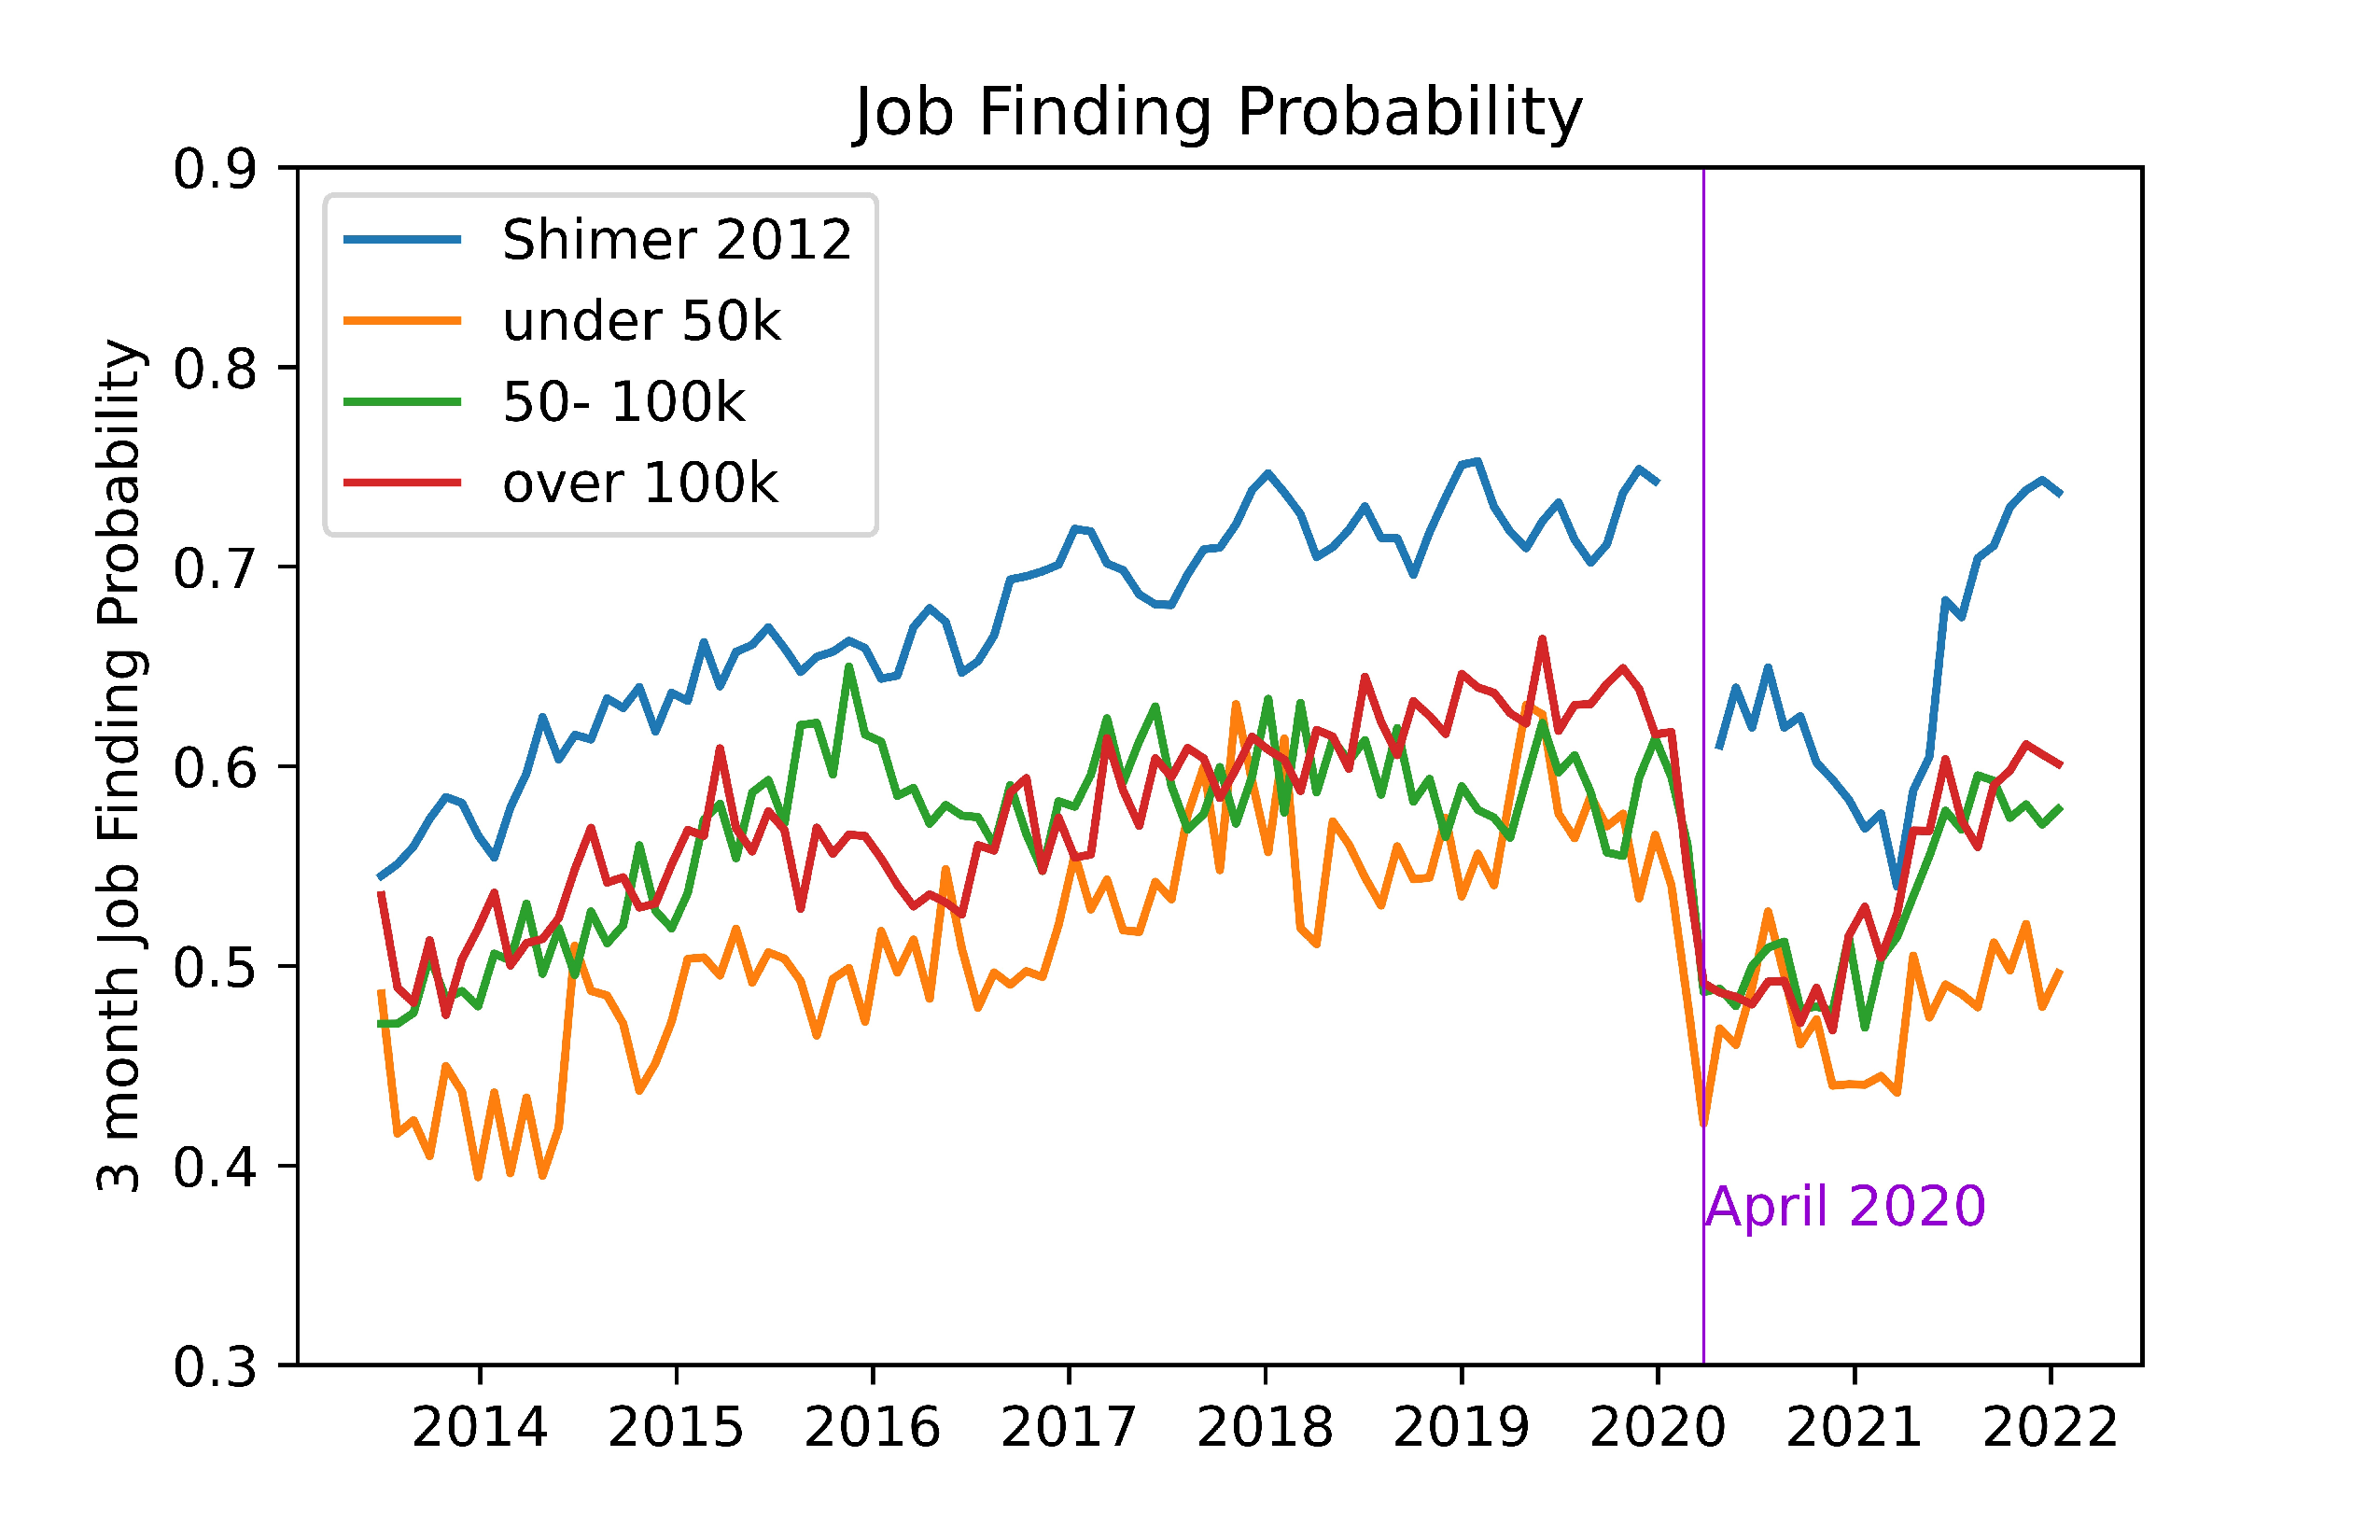
\includegraphics[scale=.26]{\FigDir/HetJF}
    \caption{Comparison of expectations of 3 month job finding across Income Groups. }
\end{figure} 


It may also be interesting to explore the consequences of heterogeneous beliefs across income (see figure 4 for a plot of expectations of job finding across income). Given households with lower levels of liquidity are more sensitive to fluctuations in unemployment risk (\cite{heathcote2018wealth}), it may be interesting to investigate the interaction between heterogeneous beliefs in job transition probabilities and distribution of wealth.  If low income households face sharper changes in unemployment risks than middle and high income households, then the change in aggregate consumption would be amplified relative to a baseline HANK model where all households face the same unemployment prospects as the low income households would have an even stronger precautionary savings motive.









%\providecommand{\figName}{GIPRM1}
%\providecommand{\figFile}{GIPRM1}
%\hypertarget{\figFile}{}
%\hypertarget{\figName}{}
%\begin{figure}[tbp]
%\centerline{\includegraphics[scale=.35]{\FigDir/\figFile}}
%\caption{Monetary Policy Shock}
%\label{fig:\figFile}
%\end{figure}


%%
%\renewcommand{\figFile}{GIPRM2}
%\hypertarget{\figFile}{}  
%\begin{figure}[tbp]
%\centerline{\includegraphics[scale=.35]{\FigDir/\figFile}}
%\caption{Monetary Policy Shock}
%\label{fig:\figFile}
%\end{figure}
%%


\clearpage\vfill\eject







%%Now let $v(m_{it}, c_{it}) = \frac{c_{i t}^{1-\rho}}{1 -\rho} - \varphi \frac{n_{it}^{1+v}}{1+v} + \beta_{i}\not D \mathrm{E}_{t}[\psi_{it+1}^{1-\rho} V(m_{it+1})] $ and let $c_{it}(m_{it})$ denote the solution to the original dynamic problem.  \\ 

%%Note $ \frac{ \partial v(m_{it},c_{it}(m_{it}))}{\partial m} =  \beta_{i}\not D \mathrm{E}_{t}[\psi_{it+1}^{1-\rho} V'(m_{it+1})] $ \\

%%Then $$ V(m_{it}) = v(m_{it}, c_{it}(m_{it})$$ 

%%$$ V'(m_{it}) = \frac{ \partial v(m_{it},c_{it}(m_{it}))}{\partial m}$$ 

%%Which leads to the envelope condition \\

%%$$V'(m_{it}) =  \beta_{i}\not D \mathrm{E}_{t}[\psi_{it+1}^{1-\rho} V'(m_{it+1})] $$





%\bibliography{\econtexRoot/BufferStockTheory,economics}

\bibliography{\econtexRoot/REF}







\end{document}
